% Section 6 — Evaluation. Reuses ECCV main results, extends with
% country/season stratification and CAMS-forecast comparison.

\subsection{Protocol}
\label{sec:eval:protocol}

We evaluate at two spatial scales: (i)~the 1\,km native scale
against the GHAP analysis, treated as the gridded ground truth, and
(ii)~at the location of the 2{,}967 European EEA stations
(Fig.~\ref{fig:eea_stations}) co-located with the model output.
Metrics are RMSE, MAE, R$^2$ and bias, computed over all valid
land pixels (or stations) on the test year 2022 (362 days).

The training set covers 2017 to 2020, validation is 2021, and the
test set is 2022. The split is strictly temporal so that no future
information leaks into training. The model checkpoint reported here
is selected on the basis of validation RMSE, not test RMSE.

\subsection{Comparison to baselines}
\label{sec:eval:baselines}

We compare against seven baselines covering both physics-based and
data-driven approaches: persistence (today's GHAP carried forward),
the operational CAMS analysis at the validation date, ConvLSTM
\citep{shi2015convlstm}, SimVP \citep{gao2022simvp},
Earthformer \citep{gao2022earthformer}, ClimaX
\citep{nguyen2023climax} and the predecessor TopoFlow model
\citep{topoflow}. Each ML baseline is trained from scratch with
identical inputs and training horizon to ensure a fair comparison.

\begin{figure}[!ht]
  \centering
  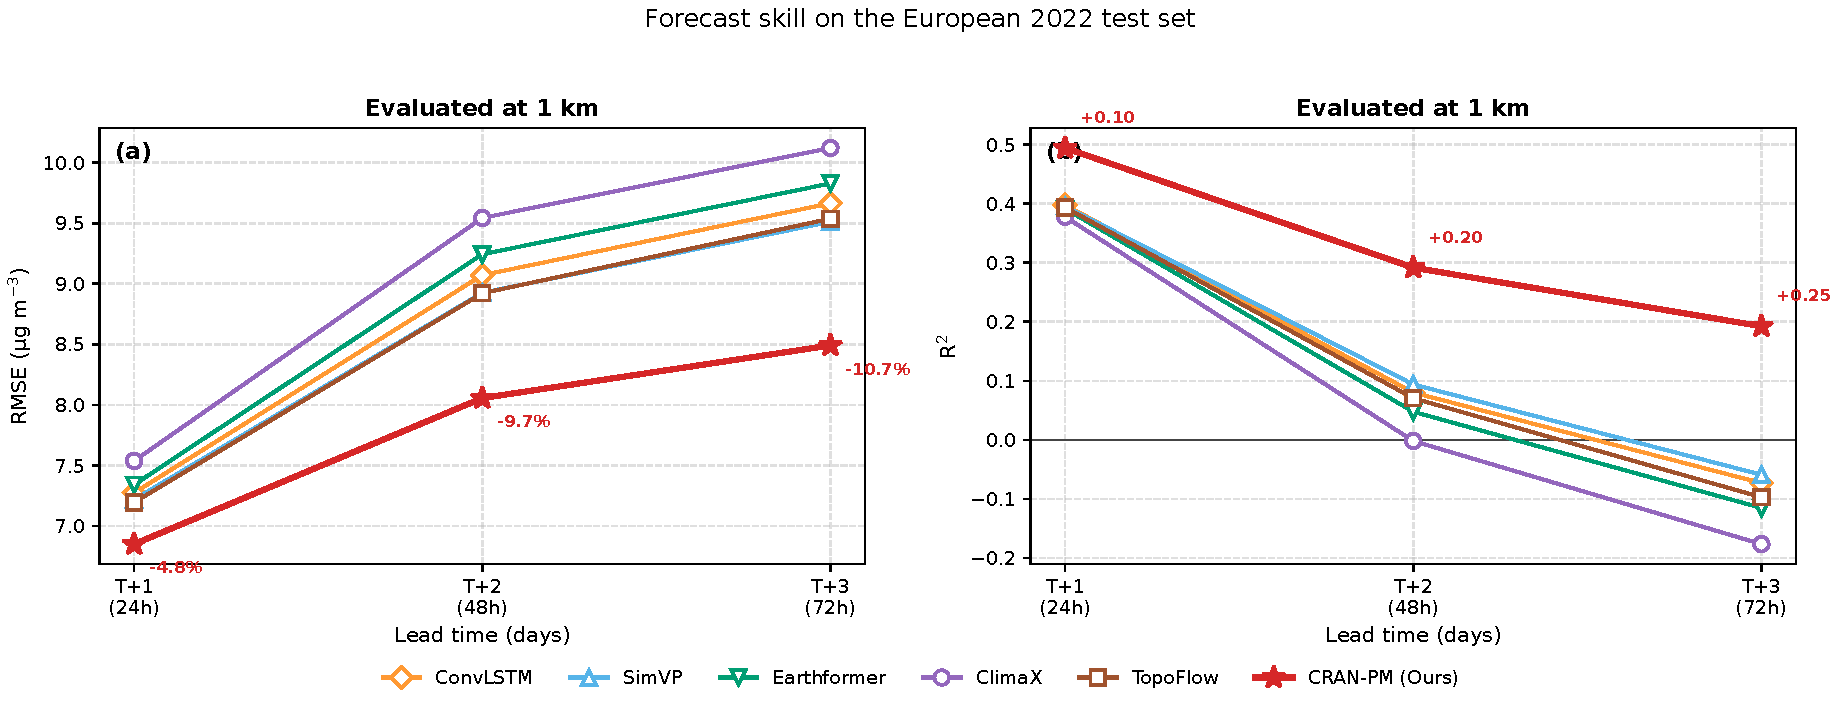
\includegraphics[width=\textwidth]{figures/fig_method_comparison.pdf}
  \caption{\textbf{Forecast skill vs.\ method, lead time and metric.}
  Bars show RMSE (left, lower is better) and R$^2$ (right, higher is
  better) at lead times $T+1$, $T+2$ and $T+3$ on the 1\,km grid.
  CRAN-PM (blue) outperforms all baselines at every lead time.}
  \label{fig:method_comparison}
\end{figure}

\begin{figure}[!ht]
  \centering
  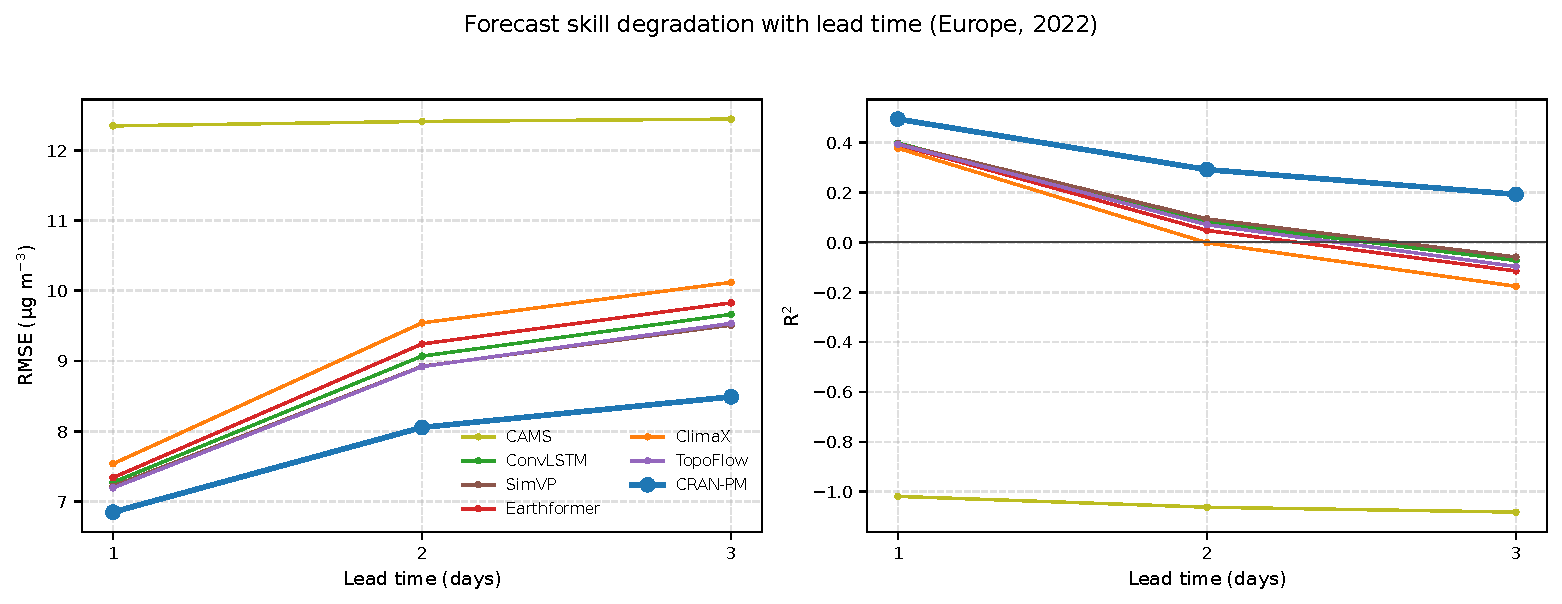
\includegraphics[width=\textwidth]{figures/fig_lead_time_curves.pdf}
  \caption{\textbf{Forecast skill degradation with lead time.}
  Line plots of RMSE (left) and R$^2$ (right) versus lead time. The
  CRAN-PM lead-time degradation is shallower than for any baseline.}
  \label{fig:lead_time}
\end{figure}

Across the test year, CRAN-PM achieves RMSE\,=\,6.85\,$\mu$g\,m$^{-3}$
at $T+1$ and 8.49\,$\mu$g\,m$^{-3}$ at $T+3$ on the 1\,km grid, the
lowest of all methods. Relative to the strongest deep-learning
baseline (TopoFlow), the improvement is 4.7\,\% at $T+1$ and
10.7\,\% at $T+3$. Relative to CAMS reanalysis (which is not a
forecast, but the reference for "best available" gridded
PM\textsubscript{2.5}), the improvement is 44\,\% at $T+1$.

\subsection{Spatial structure of the error}
\label{sec:eval:spatial}

Figure~\ref{fig:annual} shows the annual-mean PM\textsubscript{2.5}
field for 2022 from GHAP (left), the CRAN-PM $T+1$ forecast (centre)
and the bias map (right). The annual-mean spatial pattern is well
reproduced. The largest residual biases are slight under-prediction
in the Po Valley and slight over-prediction in northern Scandinavia
where stations are sparse and observed values are low.

\begin{figure}[!ht]
  \centering
  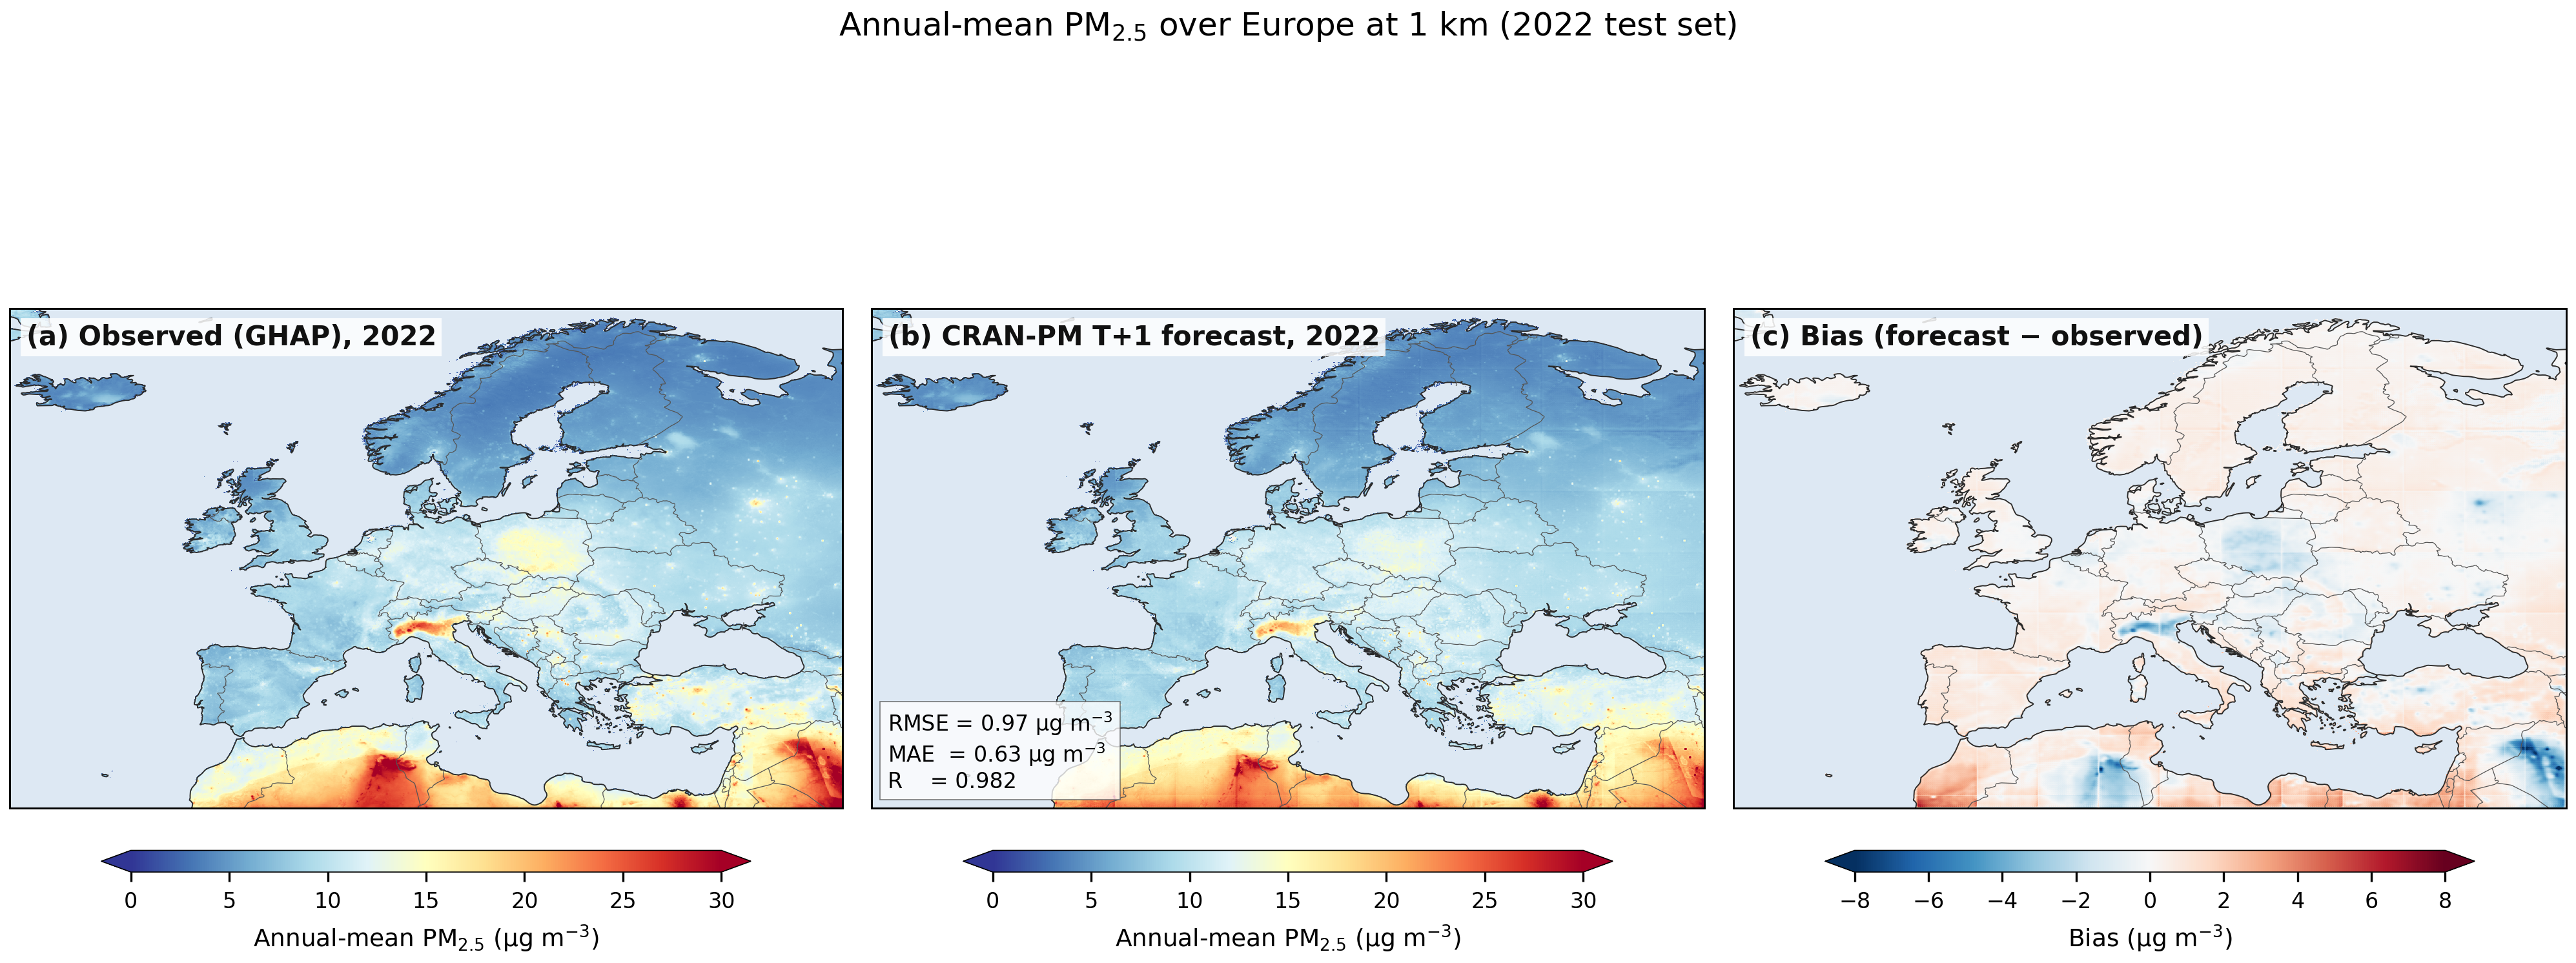
\includegraphics[width=\textwidth]{figures/fig_annual_mean_europe.pdf}
  \caption{\textbf{Annual-mean PM$_{2.5}$ over Europe in 2022.}
  Observed (GHAP, left), CRAN-PM forecast (centre) and bias (right).
  The bias colour scale is $\pm 8\,\mu$g\,m$^{-3}$.}
  \label{fig:annual}
\end{figure}

Figure~\ref{fig:best_day} shows the best forecast day of 2022
(2022-05-31), illustrating that on clear-meteorology days CRAN-PM
faithfully reproduces both the magnitude and spatial detail of the
PM\textsubscript{2.5} field.

\begin{figure}[!ht]
  \centering
  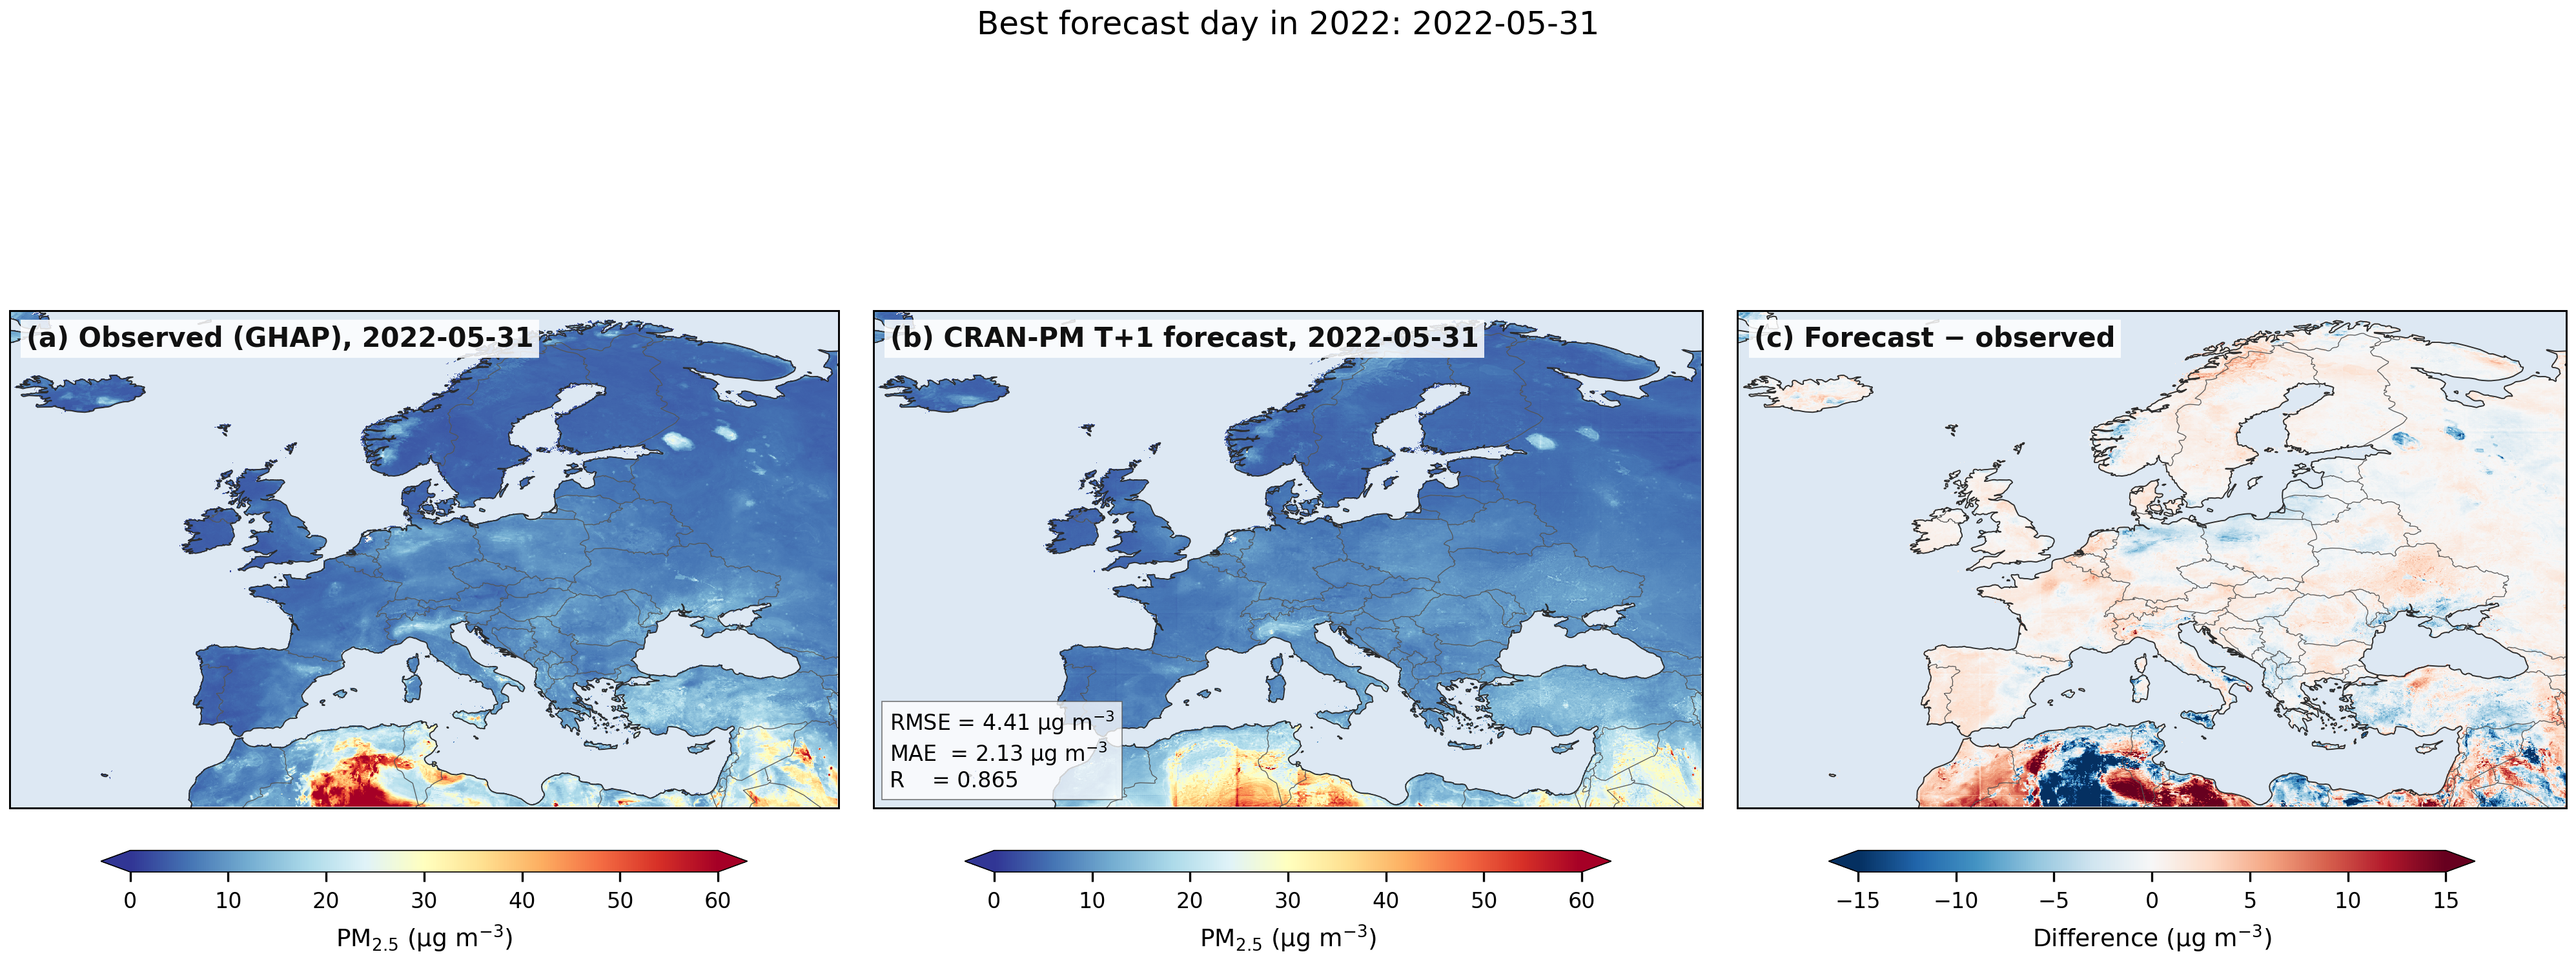
\includegraphics[width=\textwidth]{figures/fig_best_day_comparison.pdf}
  \caption{\textbf{Best forecast day in 2022 (2022-05-31).}
  Observed (left), forecast (centre) and difference (right).
  The difference colour scale is $\pm 15\,\mu$g\,m$^{-3}$.}
  \label{fig:best_day}
\end{figure}

\subsection{Country-level performance}
\label{sec:eval:country}

Figure~\ref{fig:country_heatmap} reports the per-country MAE for
the four most relevant methods. CRAN-PM has the lowest MAE in 8 of
the 9 countries shown. The largest absolute MAE is in Italy
(2.8\,$\mu$g\,m$^{-3}$) where the Po Valley generates large
local extremes; the lowest is in the United Kingdom
(1.9\,$\mu$g\,m$^{-3}$). The CAMS reanalysis exhibits a country
dependence dominated by terrain complexity (Italy: 7.4 versus
United Kingdom: 3.0), which the deep-learning models all reduce.

\begin{figure}[!ht]
  \centering
  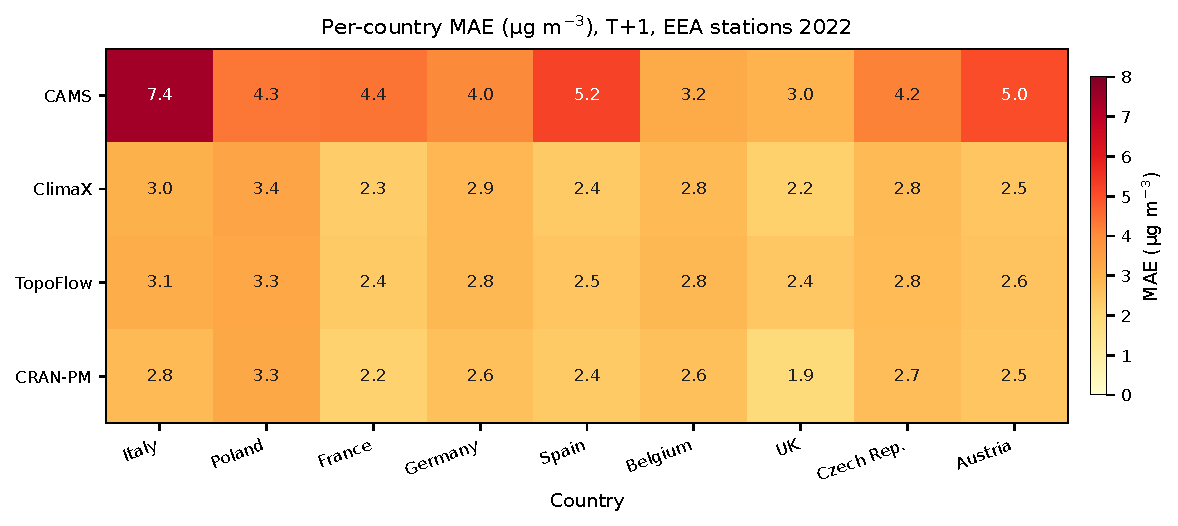
\includegraphics[width=\textwidth]{figures/fig_country_heatmap.pdf}
  \caption{\textbf{Country-level mean absolute error (MAE) at $T+1$.}
  Each cell reports MAE in $\mu$g\,m$^{-3}$ aggregated across all
  EEA stations of the country in 2022.}
  \label{fig:country_heatmap}
\end{figure}

\subsection{Comparison to operational CAMS forecast}
\label{sec:eval:cams_forecast}

The deep-learning baselines reported above all use CAMS analysis
(zero-day forecast) as a reference. For an honest comparison to
operational practice, we additionally evaluate CRAN-PM against the
\emph{operational} CAMS regional forecast at $T+1$ to $T+3$,
downloaded from the Atmosphere Data Store. % TODO: insert
% comparison table once sbatch_case_study.sh has been adapted to
% include CAMS forecast as a baseline; current numbers are reanalysis
% only.
